% !TEX TS-program = pdfLaTeX+shellescape
% !TEX encoding = UTF-8 Unicode

\documentclass{standalone}
\usepackage{pgfplots}
\pgfplotsset{compat=1.17}

\begin{document}
    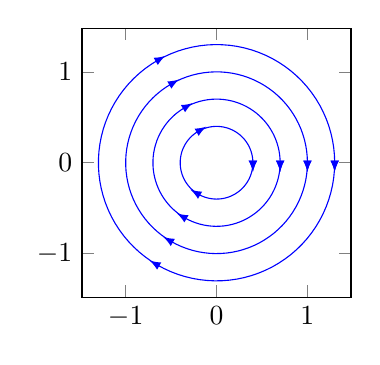
\begin{tikzpicture}[baseline]
        \begin{axis}[
            scale=0.6, % scale
            % view = {0}{90},
            xmin=-1.48,xmax=1.48,ymin=-1.48,ymax=1.48, % range of plot
            % legend style={at={(axis cs: 1,0)}, anchor=south east}, % position of legends
            % unit vector ratio = {1, 1, 1}, % aspect ratio
            unit vector ratio = {1, 1}, % aspect ratio
            % axis lines = box, % middle or box
            %axis x line = bottom, % top, middle, bottom, none: axis x line* = ... removes arrow heads
            %axis y line = left, % left, center, right, none: axis y line* = ... removes arrow heads
            %xlabel = {$x$}, ylabel = {$y$}, % axis labels 
        ]
            % \addplot3[blue, quiver={u={y}, v={-x}}, domain=-1.5:1.5, y domain=-1.5:1.5, samples=12, -latex] (x, y, 0);
            \addplot[blue, domain=0:360, samples=100]({1.3*cos(x)}, {1.3*sin(x)});
            \addplot[blue, domain=0:360, samples=100]({cos(x)}, {sin(x)});
            \addplot[blue, domain=0:360, samples=100]({0.7*cos(x)}, {0.7*sin(x)});
            \addplot[blue, domain=0:360, samples=100]({0.4*cos(x)}, {0.4*sin(x)});
            \addplot[blue, variable=\t, samples=4, domain=0:360, -latex, quiver={u={sin(t)}, v={-cos(t)}, scale arrows=0.1}]({1.3*cos(t)}, {1.3*sin(t)});
            \addplot[blue, variable=\t, samples=4, domain=0:360, -latex, quiver={u={sin(t)}, v={-cos(t)}, scale arrows=0.1}]({cos(t)}, {sin(t)});
            \addplot[blue, variable=\t, samples=4, domain=0:360, -latex, quiver={u={sin(t)}, v={-cos(t)}, scale arrows=0.1}]({0.7*cos(t)}, {0.7*sin(t)});
            \addplot[blue, variable=\t, samples=4, domain=0:360, -latex, quiver={u={sin(t)}, v={-cos(t)}, scale arrows=0.1}]({0.4*cos(t)}, {0.4*sin(t)});
        \end{axis}
    \end{tikzpicture}
\end{document}